\documentclass[12pt,a4paper]{article}

\usepackage{fontspec}
\setmainfont{Times New Roman}
\newfontfamily\cyrillicfont{Times New Roman}
\newfontfamily\cyrillicfontsf{Times New Roman}
\newfontfamily\cyrillicfonttt[Scale=0.9]{Courier New}

\usepackage{polyglossia}
\setdefaultlanguage{russian}
\setotherlanguage{english}

\usepackage{amsmath}
\usepackage{graphicx}
\usepackage{color}
\usepackage{hyperref}
\usepackage[left=3cm,right=1.5cm,top=2cm,bottom=2cm]{geometry}
\usepackage{indentfirst}
\usepackage{longtable}
\usepackage{booktabs}
\usepackage{float}
\usepackage{listings}
\usepackage{xcolor}

\lstset{
    basicstyle=\ttfamily\small,
    breaklines=true,
    frame=single,
    backgroundcolor=\color{gray!10},
    keywordstyle=\color{blue},
    commentstyle=\color{green!50!black},
    stringstyle=\color{red!60!black},
}

\hypersetup{
    colorlinks=true,
    linkcolor=blue,
    urlcolor=blue,
}

\begin{document}

\begin{titlepage}
    \centering
    {\fontsize{14pt}{16pt}\selectfont МОСКОВСКИЙ АВИАЦИОННЫЙ ИНСТИТУТ\\(НАЦИОНАЛЬНЫЙ ИССЛЕДОВАТЕЛЬСКИЙ УНИВЕРСИТЕТ)}\\[0.5cm]
    {\fontsize{12pt}{14pt}\selectfont Институт №8 «Компьютерные науки и прикладная математика»}\\[4cm]

    {\fontsize{16pt}{18pt}\selectfont \textbf{Лабораторные работы}}\\
    {\fontsize{14pt}{16pt}\selectfont \textbf{по курсу «Информационный поиск»}}\\[0.3cm]
    {\fontsize{12pt}{14pt}\selectfont Тема: Криптовалюты и блокчейн (англ.)}\\[4cm]

    \vfill
    \begin{flushright}
        \begin{minipage}{0.51\textwidth}
            Выполнил: Юнусов Р. К. \\
            Группа: М80-410Б-22\\
            Преподаватель: Кухтичев Антон Алексеевич
        \end{minipage}
    \end{flushright}

    \vfill
    {\large Москва, 2026}
\end{titlepage}

\tableofcontents
\newpage

%% ========== ЛР 1 ==========
\section{Лабораторная работа №1. Добыча корпуса документов}

\subsection{Задание}
Скачать корпус документов единой тематики, изучить его характеристики,
выделить текст, найти существующие поисковые системы для данного набора.
Источников должно быть не менее двух. Объём~--- не менее 30\,000 статей.

\subsection{Описание метода}
Для исследования выбрана тема <<Криптовалюты и блокчейн>> на английском языке.
Корпус собран из трёх независимых онлайн-изданий:
\begin{itemize}
    \item \textbf{CoinTelegraph} (cointelegraph.com)~--- одно из крупнейших медиа о криптоиндустрии;
    \item \textbf{CryptoSlate} (cryptoslate.com)~--- аналитический портал о криптовалютах и блокчейне;
    \item \textbf{Bitcoin Magazine} (bitcoinmagazine.com)~--- старейшее издание о Bitcoin.
\end{itemize}

Документы представляют собой HTML-страницы с текстовым контентом, метаинформацией
(заголовок, дата публикации, автор) и мультимедиа. Из каждой страницы извлекается
заголовок и основной текст.

Существующие поисковые системы по данным источникам:
\begin{itemize}
    \item Google с ограничением \texttt{site:cointelegraph.com};
    \item Встроенный поиск CoinTelegraph и CryptoSlate.
\end{itemize}

Примеры поисковых запросов к Google: \texttt{site:cointelegraph.com bitcoin ETF},
\texttt{site:cryptoslate.com ethereum merge}. Встроенные поисковики иногда не поддерживают
булеву логику и не показывают релевантность результатов.

\subsection{Реализация}
Написан асинхронный краулер на Python с использованием \texttt{aiohttp} и \texttt{BeautifulSoup}.
Обнаружение URL происходит через sitemap каждого источника. Конфигурация задаётся
через YAML-файл (\texttt{crawler/config.yaml}).

\subsection{Результаты}

\begin{table}[H]
\centering
\begin{tabular}{ll}
\toprule
\textbf{Показатель} & \textbf{Значение} \\
\midrule
Количество документов & 33\,290 \\
Количество источников & 3 \\
Суммарный объём текста & 132{,}8 МБ \\
Средний размер документа & 4\,344 байт \\
Средний объём текста & 4\,183 байт \\
Минимальный объём текста & 201 байт \\
Максимальный объём текста & 331\,878 байт \\
\bottomrule
\end{tabular}
\end{table}

\subsection{Выводы}
Собранный корпус содержит 33\,290 документов из трёх источников на тему
криптовалют и блокчейна. Объём текста составляет 132{,}8 МБ, что достаточно
для построения полноценного поискового индекса и проверки алгоритмов поиска.

%% ========== ЛР 2 ==========
\section{Лабораторная работа №2. Поисковый робот}

\subsection{Задание}
Написать поисковый робот, получающий путь до YAML-конфига, сохраняющий документы
в базу данных, с поддержкой остановки и продолжения обкачки.

\subsection{Описание метода}
Поисковый робот реализован на Python с использованием асинхронной библиотеки
\texttt{aiohttp} для параллельной загрузки страниц. Парсинг HTML выполняется
с помощью \texttt{BeautifulSoup} (парсер \texttt{lxml}).

Обнаружение URL-адресов происходит через XML Sitemap каждого источника.
Краулер рекурсивно обходит подсайтмапы (до 80 штук) и собирает все доступные ссылки.

\subsection{Реализация}
Конфигурация задаётся через файл \texttt{crawler/config.yaml}:

\begin{lstlisting}[language=Python]
db:
  host: localhost
  port: 27017
  name: crypto_news
sources:
  - name: cointelegraph
    sitemap: https://cointelegraph.com/sitemap.xml
    domain: cointelegraph.com
    target: 15000
\end{lstlisting}

Документы сохраняются в MongoDB со следующими полями:
\begin{itemize}
    \item \texttt{url}~--- нормализованный URL;
    \item \texttt{raw\_html}~--- сырой HTML-текст;
    \item \texttt{title}~--- заголовок;
    \item \texttt{text}~--- извлечённый текст;
    \item \texttt{source}~--- название источника;
    \item \texttt{crawl\_timestamp}~--- дата обкачки (Unix timestamp);
    \item \texttt{content\_hash}~--- MD5-хеш для определения изменений.
\end{itemize}

Робот может быть остановлен и возобновлён: при повторном запуске он пропускает уже
сохранённые URL. Переобкачка реализуется через сравнение \texttt{content\_hash}.

\subsection{Результаты}
\begin{table}[H]
\centering
\begin{tabular}{ll}
\toprule
\textbf{Показатель} & \textbf{Значение} \\
\midrule
CoinTelegraph & 14\,731 документ \\
CryptoSlate & 11\,410 документов \\
Bitcoin Magazine & 7\,292 документа \\
Итого & 33\,290 \\
Concurrency & 80 параллельных соединений \\
Общее время обкачки & $\approx$35 мин \\
\bottomrule
\end{tabular}
\end{table}

\subsection{Выводы}
Асинхронный краулер позволил собрать более 33 тысяч документов за 35 минут
благодаря высокому параллелизму (80 одновременных соединений) и использованию
сайтмапов для обнаружения URL.

%% ========== ЛР 3 ==========
\section{Лабораторная работа №3. Токенизация}

\subsection{Задание}
Реализовать разбиение текстов документов на токены, описать правила токенизации,
привести статистику.

\subsection{Описание метода}
Токенизация реализована на C++ (STL разрешён для данного этапа). Правила:
\begin{enumerate}
    \item Разделение по пробелам и знакам пунктуации;
    \item Приведение к нижнему регистру;
    \item Минимальная длина токена~--- 2 символа;
    \item Удаление чисто цифровых токенов;
    \item Апострофы внутри слов сохраняются (напр. \texttt{don't}).
\end{enumerate}

\subsection{Реализация}
Файл \texttt{core/tokenizer.cpp}. Обрабатывает каждый файл из каталога корпуса:
пропускает первые две строки (заголовок, URL), оставшийся текст разбивает на токены
по указанным правилам. Результат записывается в файл \texttt{tokens.txt}~--- по одному
токену на строку.

\subsection{Результаты}
\begin{table}[H]
\centering
\begin{tabular}{ll}
\toprule
\textbf{Показатель} & \textbf{Значение} \\
\midrule
Количество токенов & 20\,763\,046 \\
Уникальных токенов & 253\,465 \\
Средняя длина токена & 5{,}35 символа \\
Время токенизации & 3{,}43 с \\
Скорость & $\approx$38\,700 КБ/с \\
\bottomrule
\end{tabular}
\end{table}

\subsection{Выводы}
Токенизатор обработал 33\,290 файлов за 3{,}43 секунды со скоростью
около 38{,}7 МБ/с. Средняя длина токена~--- 5{,}35 символа, что характерно
для английского языка. Для ускорения можно использовать потоковое чтение
или многопоточную обработку.

%% ========== ЛР 4 ==========
\section{Лабораторная работа №4. Стемминг}

\subsection{Задание}
Добавить стемминг в поисковую систему.

\subsection{Описание метода}
Для стемминга используется оригинальный алгоритм Портера (1980) для английского языка.
Алгоритм состоит из пяти шагов, каждый из которых удаляет или заменяет определённые
суффиксы слова. В отличие от Snowball/Porter2, оригинальный алгоритм использует
классические правила, описанные в статье M.~F.~Porter.

Алгоритм реализован в файле \texttt{core/porter.h} на C++ без использования STL.
Ключевые функции: \texttt{measure()}~--- подсчёт <<меры>> основы (чередований
согласная-гласная), \texttt{is\_consonant()}~--- определение согласного,
\texttt{has\_vowel()}~--- наличие гласного, \texttt{cvc()}~--- проверка шаблона.

\subsection{Результаты}
\begin{table}[H]
\centering
\begin{tabular}{ll}
\toprule
\textbf{Показатель} & \textbf{Значение} \\
\midrule
Уникальных токенов (до стемминга) & 253\,465 \\
Уникальных основ (после стемминга) & 223\,983 \\
Сокращение словаря & $\approx$11{,}6\% \\
\bottomrule
\end{tabular}
\end{table}

Примеры работы стеммера:
\begin{itemize}
    \item \texttt{mining} $\rightarrow$ \texttt{mine}
    \item \texttt{transactions} $\rightarrow$ \texttt{transact}
    \item \texttt{cryptocurrency} $\rightarrow$ \texttt{cryptocurr}
    \item \texttt{decentralized} $\rightarrow$ \texttt{decentr}
\end{itemize}

\subsection{Выводы}
Стемминг позволил сократить словарь на 11{,}6\%, объединив различные
словоформы в единую основу. Это повышает полноту поиска: запрос \texttt{mine}
находит документы со словами \texttt{mining}, \texttt{mined}, \texttt{miner}.

%% ========== ЛР 5 ==========
\section{Лабораторная работа №5. Закон Ципфа}

\subsection{Задание}
Построить график распределения терминов по частотностям в логарифмической
шкале, наложить закон Ципфа.

\subsection{Описание метода}
Закон Ципфа утверждает, что частота $f$ слова обратно пропорциональна его рангу $r$:
$f(r) = C / r$, где $C$~--- константа, равная частоте самого частого слова.

Для построения графика используется скрипт \texttt{scripts/zipf.py} (Python, matplotlib).
По оси X~--- ранг терма, по оси Y~--- его частота, обе оси в логарифмическом масштабе.

\subsection{Результаты}

\begin{figure}[H]
    \centering
    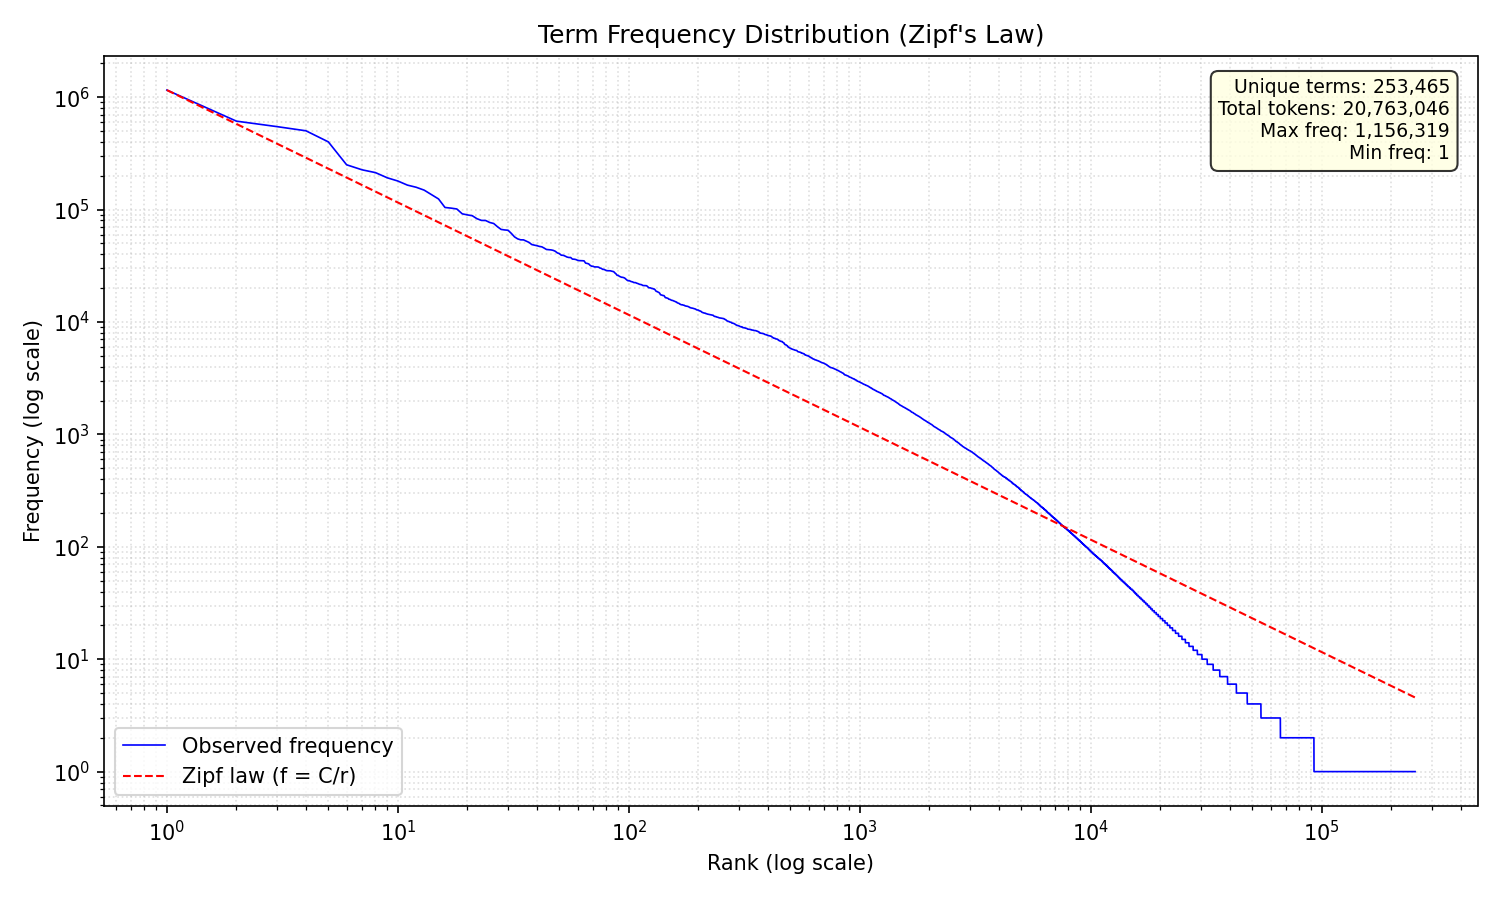
\includegraphics[width=0.9\textwidth]{screenshots/zipf_plot.png}
    \caption{Распределение терминов по частотностям (закон Ципфа), 253\,465 уникальных терминов}
    \label{fig:zipf}
\end{figure}

Наблюдаемое распределение близко к теоретическому закону Ципфа.
Расхождения наблюдаются:
\begin{itemize}
    \item В области низких рангов~--- частые служебные слова (\texttt{the}, \texttt{to}, \texttt{of})
          чуть превышают теоретическую прямую;
    \item В области высоких рангов~--- редкие технические термины
          (\texttt{defi}, \texttt{stablecoin}) отклоняются вниз из-за специфичности корпуса.
\end{itemize}

\subsection{Выводы}
Распределение частот терминов в корпусе криптовалютных новостей хорошо согласуется
с законом Ципфа. Отклонения объясняются тематической специализацией корпуса.

%% ========== ЛР 6 ==========
\section{Лабораторная работа №6. Булев индекс}

\subsection{Задание}
Построить поисковый индекс в бинарном формате, пригодный для булева поиска.

\subsection{Описание метода}
Индекс реализован на C++ без STL с использованием собственных структур данных:

\begin{itemize}
    \item \textbf{Динамический массив} (\texttt{vec.h}, структура \texttt{Vec})~---
          массив с автоматическим увеличением ёмкости (начальная~--- 32 элемента, рост~--- $\times$2).
          Сортировка~--- merge sort (стабильная, $O(n \log n)$);
    \item \textbf{Хеш-таблица} (\texttt{map.h}, структура \texttt{Map})~---
          open addressing с linear probing, хеш-функция FNV-1a
          (offset basis 2\,166\,136\,261, prime 16\,777\,619),
          начальный размер~--- 200\,003 бакета, load factor~--- 0{,}7;
    \item \textbf{Строковые утилиты} (\texttt{mystr.h})~---
          \texttt{str\_len}, \texttt{str\_dup}, \texttt{str\_cmp}, \texttt{to\_lower} и др.
\end{itemize}

\subsubsection{Формат индекса}
Бинарный файл \texttt{index.bin} с магическим числом \texttt{YIDX}:

\begin{table}[H]
\centering
\begin{tabular}{lll}
\toprule
\textbf{Секция} & \textbf{Смещение} & \textbf{Описание} \\
\midrule
Заголовок & 0 & Magic (4B), version (4B), num\_terms (4B), num\_docs (4B), \\
          &   & fwd\_offset (8B), dict\_offset (8B), post\_offset (8B)~--- 40 байт \\
Прямой индекс & fwd\_offset & Для каждого документа: url\_len (2B), url, \\
              &            & title\_len (2B), title, source\_len (2B), source \\
Постинги & post\_offset & Для каждого терма: отсортированные doc\_id (4B) \\
Словарь & dict\_offset & Для каждого терма: term\_len (1B), term, \\
        &             & posting\_offset (8B), posting\_count (4B) \\
\bottomrule
\end{tabular}
\end{table}

Формат предусматривает расширение: поле version позволяет добавлять новые секции.

\subsection{Результаты}
\begin{table}[H]
\centering
\begin{tabular}{ll}
\toprule
\textbf{Показатель} & \textbf{Значение} \\
\midrule
Количество документов & 33\,290 \\
Количество термов & 223\,983 \\
Количество постингов & 9\,401\,651 \\
Размер индекса & 46 МБ \\
Средняя длина терма & 5{,}35 символа \\
Время индексации & 7{,}28 с \\
Скорость & $\approx$4\,573 доков/с \\
\bottomrule
\end{tabular}
\end{table}

\subsection{Выводы}
Индекс построен за 7{,}28 секунды. Использование хеш-таблицы с open addressing
и FNV-1a обеспечивает быстрый поиск терма ($O(1)$ в среднем). Merge sort
гарантирует стабильность сортировки постингов. При увеличении корпуса в 10 раз
основным ограничением станет объём оперативной памяти.

%% ========== ЛР 7 ==========
\section{Лабораторная работа №7. Булев поиск}

\subsection{Задание}
Реализовать ввод поисковых запросов и их выполнение над индексом, веб-сервис и CLI.

\subsection{Описание метода}
Парсер булевых запросов реализован по алгоритму shunting-yard (алгоритм Дейкстры).
Используются два стека~--- операндов и операторов. Приоритет операций:
\texttt{NOT}~$>$~\texttt{AND}~$>$~\texttt{OR}. Пробел интерпретируется как \texttt{AND}.

Поддерживаемый синтаксис:
\begin{itemize}
    \item \texttt{\&\&} или пробел~--- логическое И;
    \item \texttt{||}~--- логическое ИЛИ;
    \item \texttt{!}~--- логическое НЕ;
    \item Скобки для группировки.
\end{itemize}

Реализация на C++ (\texttt{core/search\_cli.cpp}) без STL. Поиск терма выполняется
бинарным поиском по отсортированному словарю. Операции над списками постингов~---
двухуказательное слияние ($O(n+m)$).

\subsection{Реализация}

\subsubsection{CLI}
Утилита \texttt{search\_cli} получает путь к индексу и выполняет запросы со
стандартного ввода. Поддерживает флаги \texttt{-{}-json} и \texttt{-{}-limit}.

\subsubsection{Веб-сервис}
Веб-сервис реализован на Flask (Python). Два маршрута: \texttt{GET /}~--- форма
ввода, \texttt{GET /search?q=...}~--- страница результатов (50 на страницу, пагинация).
Для выполнения запроса вызывается \texttt{search\_cli} через \texttt{subprocess}.

\begin{figure}[H]
    \centering
    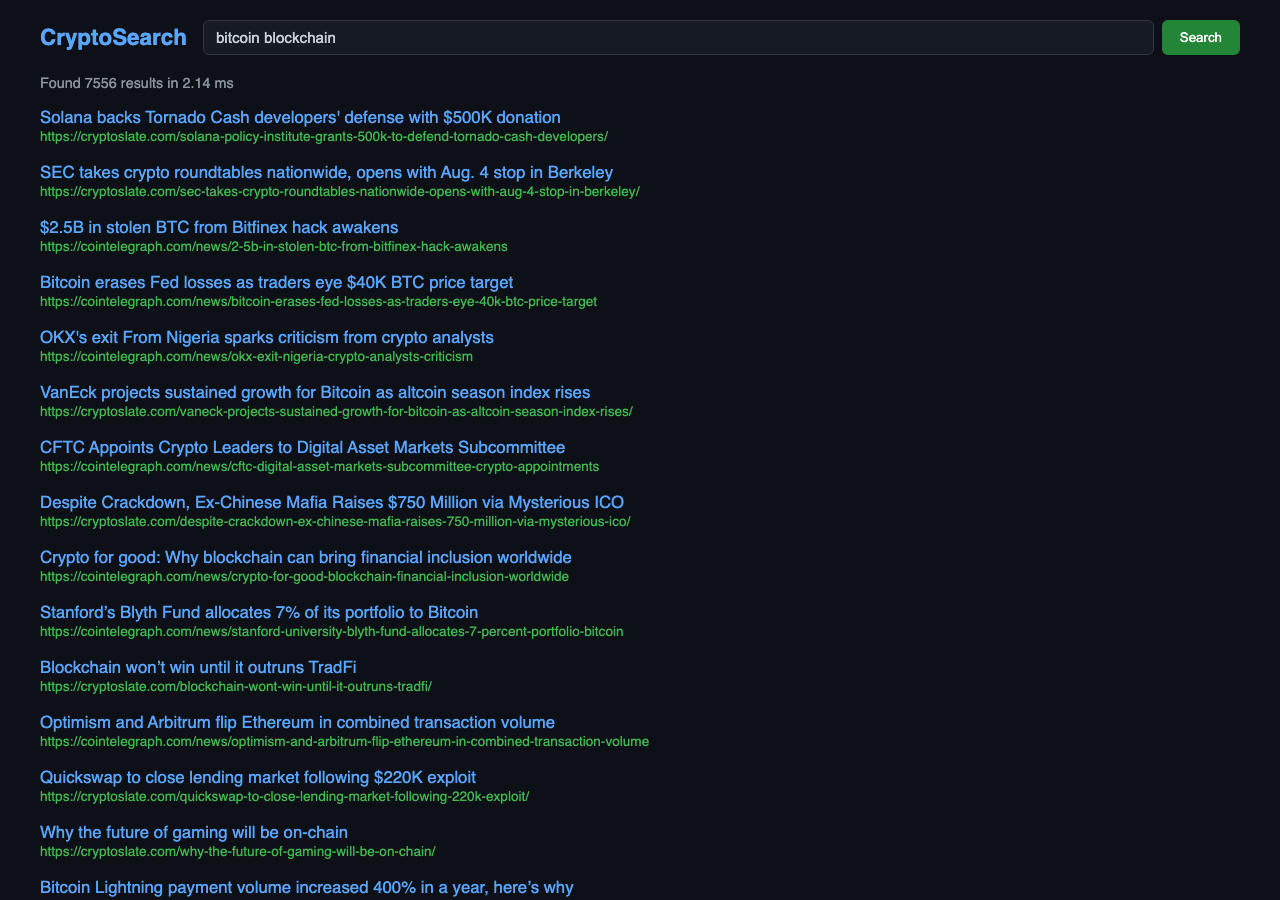
\includegraphics[width=0.95\textwidth]{screenshots/web_search.png}
    \caption{Скриншот поисковой выдачи (запрос <<bitcoin blockchain>>, 7\,556 результатов, 1{,}64 мс)}
    \label{fig:web_real}
\end{figure}

\subsection{Результаты}
\begin{table}[H]
\centering
\begin{tabular}{ll}
\toprule
\textbf{Запрос} & \textbf{Результат (время)} \\
\midrule
\texttt{bitcoin} & 21\,711 (1{,}24 мс) \\
\texttt{ethereum || solana} & 8\,196 (1{,}58 мс) \\
\texttt{bitcoin \&\& !ethereum} & 17\,633 (9{,}96 мс) \\
\texttt{bitcoin blockchain} & 7\,556 (1{,}64 мс) \\
\bottomrule
\end{tabular}
\end{table}

Запросы с оператором \texttt{NOT} выполняются дольше, так как требуют
обход всего множества документов.

\subsection{Выводы}
Поисковая система обрабатывает запросы за 1--10 мс. Алгоритм shunting-yard
корректно разбирает выражения с произвольной вложенностью скобок и
переменным числом пробелов. Веб-интерфейс на Flask обеспечивает удобный
доступ к результатам поиска с пагинацией.

%% ========== ЗАКЛЮЧЕНИЕ ==========
\section*{Заключение}
\addcontentsline{toc}{section}{Заключение}

В рамках лабораторных работ реализована полноценная поисковая система
для корпуса криптовалютных и блокчейн-новостей на английском языке:

\begin{enumerate}
    \item Собран корпус из 33\,290 документов из трёх источников (CoinTelegraph, CryptoSlate, Bitcoin Magazine);
    \item Реализован асинхронный краулер с поддержкой возобновления и переобкачки;
    \item Построен токенизатор со скоростью $\approx$38{,}7 МБ/с;
    \item Применён стемминг по алгоритму Портера, сокративший словарь на 11{,}6\%;
    \item Подтверждено соответствие корпуса закону Ципфа;
    \item Построен бинарный поисковый индекс (223\,983 терма, 9{,}4 млн постингов, 46 МБ);
    \item Реализован булев поиск с веб-интерфейсом и CLI.
\end{enumerate}

Ядро поисковой системы написано на C++ без использования STL, с собственными
реализациями динамического массива, хеш-таблицы (FNV-1a, open addressing),
стеммера Портера и парсера запросов (shunting-yard).

\end{document}
